\chapter{TINJAUAN PUSTAKA}

\section{Kajian Teori}

\subsection{Web Penetration Testing}
\textit{Web penetration testing} merupakan metode pengujian keamanan aplikasi web dengan cara mensimulasikan serangan yang dilakukan oleh penyerang. Tujuan utama dari metode ini adalah untuk mengidentifikasi kerentanan yang dapat dimanfaatkan untuk mengakses sistem secara tidak sah.

Proses \textit{penetration testing} umumnya terdiri dari beberapa tahap, yaitu:
\begin{enumerate}
    \item \textbf{\textit{Information Gathering}}: Pengumpulan informasi target.
    \item \textbf{\textit{Vulnerability Scanning}}: Pemindaian celah keamanan.
    \item \textbf{\textit{Exploitation}}: Percobaan penetrasi pada celah yang ditemukan.
    \item \textbf{\textit{Reporting}}: Pelaporan hasil pengujian.
\end{enumerate}

Pendekatan ini sangat penting dalam menjaga keamanan sistem, namun memiliki keterbatasan jika dilakukan secara manual, seperti tidak efisien dan bergantung pada keahlian penguji. \textit{Penetration testing} tidak hanya berfungsi sebagai metode identifikasi kerentanan, tetapi juga sebagai mekanisme evaluasi terhadap efektivitas sistem keamanan yang telah diterapkan. Dalam praktiknya, proses ini meniru pola serangan yang dilakukan oleh penyerang nyata sehingga mampu memberikan gambaran yang lebih realistis terhadap potensi risiko yang dihadapi oleh sistem (\cite{singerfriedman2014}).

\subsection{Vulnerability pada Aplikasi Web}

Kerentanan (\textit{vulnerability}) merupakan suatu kelemahan atau celah dalam desain, implementasi, operasi, maupun manajemen sistem yang dapat dieksploitasi oleh aktor ancaman (\textit{threat actor}) untuk melanggar kebijakan keamanan sistem tersebut. Pada arsitektur aplikasi web modern yang berbasis \textit{three-tier} (klien, server, dan database), kerentanan umumnya muncul akibat kegagalan dalam validasi input, sanitasi data yang tidak memadai, kesalahan konfigurasi keamanan (\textit{security misconfiguration}), serta kelemahan pada logika autentikasi dan otorisasi.

Untuk memberikan standardisasi dalam identifikasi risiko, \textit{Open Web Application Security Project} (OWASP) secara berkala merilis daftar risiko keamanan paling kritis. Berdasarkan metodologi pengujian keamanan aplikasi web, berikut adalah penjelasan rinci mengenai beberapa jenis kerentanan utama yang sering menjadi target eksploitasi:

\begin{enumerate}
    \item \textbf{\textit{SQL Injection} (SQLi)}
    
    \textit{SQL Injection} terjadi ketika data yang disuplai oleh pengguna (*user-supplied data*) langsung digabungkan ke dalam \textit{query} SQL tanpa melalui proses filtrasi atau menggunakan \textit{parameterized queries}. Akibatnya, interpreter database menginterpretasikan input tersebut sebagai perintah eksekusi, bukan sebagai data biasa. 
    
    
    
    Dampak dari serangan ini sangat fatal, meliputi kebocoran data sensitif (\textit{data exfiltration}), manipulasi atau penghapusan isi database (\textit{data tampering}), hingga pengambilalihan kontrol server database melalui fungsi \textit{stacked queries} atau \textit{command execution}.

    \item \textbf{\textit{Cross-Site Scripting} (XSS)}
    
    Kerentanan XSS terjadi ketika aplikasi web menyertakan data yang tidak terpercaya ke dalam halaman web yang dikirimkan ke \textit{browser} pengguna tanpa melakukan sanitasi atau \textit{output encoding} yang tepat. Hal ini memungkinkan penyerang untuk menyuntikkan \textit{malicious script} (umumnya berbasis JavaScript) yang akan dieksekusi oleh \textit{browser} korban dalam konteks sesi mereka. 
    
    
    
    Secara umum, XSS dibagi menjadi tiga kategori:
    \begin{itemize}
        \item \textbf{\textit{Stored XSS}}: \textit{Script} berbahaya disimpan secara permanen di server (misalnya pada database atau kolom komentar) dan dieksekusi setiap kali pengguna mengakses halaman tersebut.
        \item \textbf{\textit{Reflected XSS}}: \textit{Script} berbahaya dipantulkan dari \textit{request} HTTP (misalnya melalui parameter URL) langsung ke dalam \textit{response} tanpa disimpan.
        \item \textbf{\textit{DOM-based XSS}}: Eksekusi \textit{script} terjadi sepenuhnya di sisi klien akibat modifikasi \textit{Document Object Model} (DOM) oleh \textit{script} lokal yang tidak aman.
    \end{itemize}
    Dampak XSS meliputi pencurian token sesi (\textit{session hijacking}), pencurian kredensial melalui \textit{credential harvesting}, serta deface halaman web pada sisi klien.

    \item \textbf{\textit{Local File Inclusion} (LFI)}
    
    LFI adalah kerentanan yang terjadi ketika aplikasi web mengizinkan input dari pengguna untuk menentukan berkas yang akan dimuat atau dieksekusi secara lokal oleh server tanpa adanya validasi jalur (\textit{path validation}) yang ketat. Kerentanan ini sering ditemukan pada fungsi penanganan bahasa pemrograman web (seperti fungsi \texttt{include()}, \texttt{require()}, atau \texttt{file\_get\_contents()} pada PHP).
    
    Penyerang dapat menggunakan teknik \textit{directory traversal} (misalnya memasukkan urutan karakter \texttt{../../}) untuk membaca berkas sensitif di dalam sistem operasi server, seperti berkas konfigurasi aplikasi, \texttt{/etc/passwd} pada Linux, atau bahkan mencapai tahap \textit{Remote Code Execution} (RCE) melalui teknik \textit{log poisoning}.

    \item \textbf{\textit{Fuzzing} (Pengujian Kerentanan Otomatis)}
    
    Berbeda dengan tiga poin sebelumnya yang merujuk pada jenis celah keamanan, \textit{fuzzing} (atau \textit{fuzz testing}) merupakan teknik dan metodologi pengujian perangkat lunak yang digunakan untuk menemukan kerentanan tersembunyi secara otomatis. Proses ini dilakukan dengan cara memberikan input data yang tidak valid, tidak terduga, atau acak (\textit{malformed input}) dalam jumlah besar ke dalam titik masuk (\textit{entry point}) aplikasi web.
    
    Dalam konteks \textit{automated penetration testing}, \textit{fuzzing} digunakan untuk memicu perilaku anomali pada aplikasi, seperti \textit{error} internal server (HTTP 500), \textit{buffer overflow}, kebocoran informasi melalui pesan \textit{error}, atau \textit{unhandled exceptions}. Respons anomali inilah yang menjadi indikator kuat adanya celah keamanan yang dapat dieksploitasi lebih lanjut.
\end{enumerate}

Secara teoritis, pemahaman mendalam terhadap mekanisme dan karakteristik dari setiap kerentanan ini menjadi fondasi penting dalam merancang model keputusan (seperti pemetaan \textit{state} dan \textit{action} pada \textit{Reinforcement Learning}) untuk melakukan penetrasi atau pemindaian celah keamanan secara adaptif dan otomatis.

\subsection{Automated Penetration Testing}

\textit{Automated penetration testing} merupakan metode pengujian keamanan sistem yang menggunakan perangkat lunak untuk menjalankan rangkaian aktivitas pengujian dan mengidentifikasi kerentanan pada aplikasi atau jaringan. Sejumlah penelitian menerapkan pembelajaran penguatan untuk mengotomatisasi pengambilan keputusan selama pengujian penetrasi (\cite{ghanem2023hrl,zennaro2023}). Pendekatan ini ditujukan untuk mengurangi pekerjaan berulang, meskipun cakupan dan hasilnya bergantung pada lingkungan serta model pengujian yang digunakan.

Pada umumnya, \textit{automated penetration testing} bekerja dengan melakukan serangkaian tahapan secara otomatis, mulai dari proses \textit{information gathering}, \textit{vulnerability scanning}, analisis celah keamanan, hingga simulasi eksploitasi terhadap kerentanan yang ditemukan. Beberapa \textit{tools} yang umum digunakan dalam pendekatan ini antara lain \textit{Nmap} untuk pemetaan jaringan, \textit{Nikto} untuk pengujian keamanan web server, serta \textit{OWASP ZAP} dan \textit{Burp Suite} untuk pengujian aplikasi web. Penggunaan \textit{tools} tersebut memungkinkan proses pengujian dilakukan secara berulang dengan hasil yang lebih konsisten dibandingkan pengujian manual.

Selain meningkatkan efisiensi, \textit{automated penetration testing} juga membantu organisasi dalam melakukan pengujian keamanan secara berkala guna mendeteksi potensi kerentanan lebih dini. Pendekatan ini sangat bermanfaat pada lingkungan sistem modern yang memiliki kompleksitas tinggi dan perubahan konfigurasi yang cepat. Dengan pengujian otomatis, proses evaluasi keamanan dapat dilakukan secara kontinu sehingga membantu menjaga keamanan sistem secara lebih efektif.

Meskipun demikian, sebagian besar sistem \textit{automated penetration testing} saat ini masih menggunakan pendekatan \textit{rule-based} atau berbasis aturan yang telah ditentukan sebelumnya. Sistem hanya mampu menjalankan pola pengujian yang sudah diprogram dan cenderung kurang fleksibel dalam menghadapi kerentanan baru atau pola serangan yang dinamis. Ketika lingkungan sistem berubah atau muncul teknik serangan baru, sistem otomatis sering kali tidak dapat menyesuaikan strategi pengujiannya secara adaptif.

Keterbatasan tersebut menyebabkan proses pengujian keamanan belum sepenuhnya optimal, terutama dalam menghadapi aplikasi modern yang memiliki struktur dan perilaku yang kompleks. Oleh karena itu, diperlukan pendekatan yang lebih adaptif dan cerdas agar sistem \textit{automated penetration testing} mampu belajar dari lingkungan pengujian serta menentukan strategi pengujian yang lebih efektif secara otomatis. Salah satu pendekatan yang mulai banyak diteliti untuk mengatasi permasalahan tersebut adalah penerapan \textit{Reinforcement Learning} dalam proses \textit{penetration testing}.

\subsection{Machine Learning dalam Cybersecurity}

\textit{Machine Learning} merupakan cabang dari kecerdasan buatan (\textit{Artificial Intelligence}) yang memungkinkan sistem komputer mempelajari pola dari data dan membuat keputusan tanpa harus diprogram secara eksplisit (\cite{mitchell1997}). Pendekatan ini bekerja dengan memanfaatkan data historis untuk membangun model yang dapat mengenali pola tertentu, melakukan prediksi, maupun mengambil keputusan secara otomatis. Seiring meningkatnya kompleksitas sistem digital dan jumlah ancaman siber, \textit{machine learning} menjadi salah satu teknologi yang banyak diterapkan dalam bidang keamanan siber.

Dalam konteks \textit{cybersecurity}, \textit{machine learning} dimanfaatkan untuk mendeteksi anomali perilaku sistem, mengidentifikasi aktivitas mencurigakan, mengklasifikasikan jenis serangan, serta menganalisis log keamanan dalam jumlah besar secara otomatis. Teknologi ini mampu membantu proses identifikasi ancaman yang sulit dideteksi menggunakan metode konvensional berbasis aturan (\textit{rule-based}). Dengan mempelajari pola lalu lintas jaringan dan aktivitas pengguna, sistem dapat mengenali indikasi serangan seperti \textit{malware}, \textit{phishing}, \textit{Distributed Denial of Service} (DDoS), maupun upaya eksploitasi celah keamanan lainnya.

Penerapan \textit{machine learning} dalam keamanan siber umumnya menggunakan beberapa pendekatan utama, yaitu \textit{supervised learning}, \textit{unsupervised learning}, dan \textit{reinforcement learning}. \textit{Supervised learning} digunakan ketika data pelatihan telah memiliki label sehingga sistem dapat mempelajari hubungan antara data dan kategori serangan tertentu. Sementara itu, \textit{unsupervised learning} digunakan untuk menemukan pola atau anomali pada data yang belum memiliki label. Adapun \textit{reinforcement learning} memungkinkan agen belajar melalui interaksi langsung dengan lingkungan berdasarkan mekanisme \textit{reward} dan \textit{punishment}.

Keunggulan utama \textit{machine learning} dalam \textit{cybersecurity} terletak pada kemampuannya dalam memproses data dalam skala besar dan melakukan adaptasi terhadap pola ancaman baru. Sistem dapat terus meningkatkan performanya seiring bertambahnya data yang dipelajari. Hal ini menjadikan \textit{machine learning} lebih fleksibel dibandingkan pendekatan tradisional yang hanya mengandalkan aturan statis.

Meskipun demikian, penerapan \textit{machine learning} dalam keamanan siber juga memiliki beberapa tantangan. Kualitas dan jumlah data pelatihan sangat memengaruhi performa model yang dihasilkan. Selain itu, model yang tidak dilatih dengan baik dapat menghasilkan \textit{false positive} atau \textit{false negative} yang berpotensi mengurangi efektivitas sistem keamanan. Kompleksitas proses pelatihan dan kebutuhan sumber daya komputasi yang tinggi juga menjadi salah satu tantangan dalam implementasinya.

Dengan berbagai kemampuan tersebut, \textit{machine learning} menjadi teknologi yang menjanjikan untuk mendukung pengembangan sistem keamanan siber yang lebih adaptif, termasuk dalam bidang \textit{automated penetration testing}. Integrasi \textit{machine learning}, khususnya \textit{reinforcement learning}, diharapkan mampu meningkatkan kemampuan sistem dalam menentukan strategi pengujian keamanan secara otomatis dan dinamis sesuai kondisi lingkungan pengujian.a

\subsection{Reinforcement Learning}
\textit{Reinforcement Learning} (RL) merupakan metode pembelajaran berbasis interaksi antara agen dan lingkungan (\cite{sutton2018}). Dalam metode ini, agen belajar memilih tindakan (\textit{action}) terbaik berdasarkan umpan balik yang diterima dari lingkungan dalam bentuk \textit{reward}. Proses pembelajaran dilakukan secara bertahap melalui percobaan berulang sehingga agen dapat menemukan strategi yang paling optimal.

Komponen utama dalam \textit{Reinforcement Learning} meliputi:
\begin{enumerate}
    \item \textbf{\textit{State}}: Representasi kondisi sistem saat ini.
    \item \textbf{\textit{Action}}: Tindakan yang diambil oleh agen.
    \item \textbf{\textit{Reward}}: Nilai positif atau negatif sebagai umpan balik dari lingkungan.
    \item \textbf{\textit{Agent \& Environment}}: Subjek yang belajar dan dunia tempat agen berinteraksi.
\end{enumerate}

Hubungan antara komponen-komponen tersebut dapat digambarkan dalam suatu siklus interaksi antara agen dan lingkungan, seperti ditunjukkan pada Gambar berikut.

\begin{figure}[H]
\centering
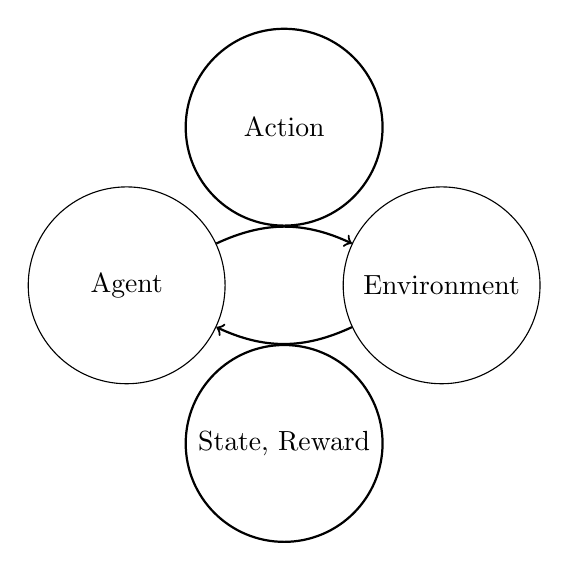
\begin{tikzpicture}[
    node distance=4cm,
    every node/.style={draw, circle, minimum size=2.5cm, align=center},
    arrow/.style={->, thick}
]
\node (agent) {Agent};
\node (env) [right of=agent] {Environment};

\draw[arrow] (agent) to[bend left=25] node[above] {Action} (env);
\draw[arrow] (env) to[bend left=25] node[below] {State, Reward} (agent);
\end{tikzpicture}
\caption{Konsep Reinforcement Learning}
\end{figure}

Gambar tersebut menunjukkan bahwa agen melakukan suatu tindakan terhadap lingkungan, kemudian lingkungan memberikan respons berupa \textit{state} baru dan \textit{reward}. Proses ini berlangsung secara terus-menerus sehingga agen dapat belajar dari pengalaman dan meningkatkan kualitas keputusan yang diambil.

Keunggulan utama \textit{Reinforcement Learning} dibandingkan metode \textit{machine learning} lainnya terletak pada kemampuannya dalam belajar melalui interaksi langsung dengan lingkungan, tanpa memerlukan dataset berlabel secara eksplisit.

\subsection{Reinforcement Learning dalam Penetration Testing}
Dalam konteks ini, RL digunakan untuk menentukan strategi pengujian secara adaptif. Agen akan memilih \textit{payload} atau tindakan tertentu, kemudian mengevaluasi hasilnya untuk meningkatkan strategi berikutnya.

Secara umum, proses penerapan \textit{Reinforcement Learning} dalam \textit{penetration testing} dapat digambarkan sebagai suatu alur interaksi antara agen, sistem target, dan mekanisme evaluasi, seperti ditunjukkan pada Gambar berikut.

\begin{figure}[H]
\centering
\begin{tikzpicture}[
    block/.style={
        draw, rectangle, rounded corners,
        minimum width=3cm, minimum height=1cm, align=center,
        fill=white
    },
    arrow/.style={->, >=stealth, thick}
]

\node[block] (agent) {RL Agent};
\node[block] (payload) [right=1cm of agent] {Payload};
\node[block] (web) [right=1cm of payload] {Web Application};

\node[block] (response) [below=1.5cm of web] {Response};
\node[block] (analyzer) [below=1.5cm of payload] {Analyzer};
\node[block] (reward) [below=1.5cm of agent] {Reward};

\draw[arrow] (agent) -- (payload);
\draw[arrow] (payload) -- (web);
\draw[arrow] (web) -- (response);
\draw[arrow] (response) -- (analyzer);
\draw[arrow] (analyzer) -- (reward);
\draw[arrow] (reward) -- (agent);

\end{tikzpicture}
\caption{Penerapan Reinforcement Learning dalam Penetration Testing}
\end{figure}

Gambar tersebut menunjukkan bahwa agen akan memilih \textit{payload} untuk dikirim ke aplikasi web. Selanjutnya, sistem akan memberikan respons yang kemudian dianalisis untuk menentukan apakah terdapat indikasi kerentanan. Hasil analisis ini digunakan untuk memberikan \textit{reward} kepada agen sebagai dasar dalam memperbaiki strategi pada langkah berikutnya.

Pendekatan ini memungkinkan eksplorasi \textit{attack path} yang lebih luas dan tidak terduga, pengambilan keputusan yang adaptif terhadap mekanisme proteksi server, serta peningkatan efisiensi pengujian melalui eliminasi tindakan yang tidak efektif.

\section{Penelitian Terkait}

\subsubsection{Literature Review}

\begin{table}[H]
\centering
\footnotesize
\renewcommand{\arraystretch}{1.2}
\setlength{\tabcolsep}{3pt}

\begin{tabularx}{\textwidth}{|c|p{3.2cm}|l|c|X|X|X|}
\hline
\textbf{No} & \textbf{Judul Penelitian} & \textbf{Peneliti} & \textbf{Tahun} & \textbf{Kelebihan} & \textbf{Kekurangan} & \textbf{Hasil} \\ \hline

1 & PentestGPT: Evaluating and Harnessing Large Language Models for Automated Penetration Testing & Deng et al. \cite{deng2024pentestgpt} & 2024 & Menggunakan LLM untuk mengotomatisasi tahapan penetration testing & Tidak menggunakan RL dan diuji pada kumpulan skenario tertentu & Menunjukkan potensi LLM untuk membantu tugas penetration testing \\ \hline

2 & Deep Reinforcement Learning for Cyber Security & Nguyen dan Reddi \cite{nguyen2023} & 2023 & Merangkum penerapan DRL dalam keamanan siber & Bersifat survei dan tidak berfokus pada web penetration testing & Memetakan pendekatan DRL untuk pertahanan dan deteksi siber \\ \hline

3 & Deep Q-Learning Based Reinforcement Learning Approach for Network Intrusion Detection & Alavizadeh et al. \cite{alavizadeh2022} & 2022 & Menerapkan deep Q-learning pada deteksi intrusi jaringan & Fokus pada deteksi, bukan eksploitasi atau penetration testing & Mengevaluasi pendekatan Q-learning untuk klasifikasi intrusi \\ \hline

4 & Hierarchical Reinforcement Learning for Efficient and Effective Automated Penetration Testing of Large Networks & Ghanem et al. \cite{ghanem2023hrl} & 2023 & Menggunakan HRL untuk membagi pengujian jaringan besar & Dievaluasi pada pemodelan jaringan, bukan aplikasi web & Menggunakan pengelompokan jaringan untuk menangani skala pengujian \\ \hline

5 & Modelling Penetration Testing with Reinforcement Learning Using Capture-the-Flag Challenges & Zennaro dan Erdodi \cite{zennaro2023} & 2023 & Membahas trade-off antara RL model-free dan pengetahuan awal & Menggunakan skenario CTF yang disederhanakan & Menunjukkan peran pengetahuan awal dalam eksplorasi agen \\ \hline

6 & GAIL-PT: An Intelligent Penetration Testing Framework with Generative Adversarial Imitation Learning & Chen et al. \cite{chen2023gailpt} & 2023 & Menggabungkan pengetahuan ahli, imitation learning, dan RL/DRL & Tidak berfokus pada aplikasi web & Melaporkan evaluasi pada host dan jaringan simulasi \\ \hline

7 & A Hierarchical Deep Reinforcement Learning Model with Expert Prior Knowledge for Intelligent Penetration Testing & Li et al. \cite{li2023hrlpt} & 2023 & Memanfaatkan prior ahli untuk membantu eksplorasi dan pembelajaran hierarkis & Berfokus pada pengujian jaringan, bukan aplikasi web & Mengusulkan model DRL hierarkis untuk penetration testing \\ \hline

8 & An Automated Penetration Testing Framework Based on Hierarchical Reinforcement Learning & Liu et al. \cite{liu2024hrlpt} & 2024 & Menggunakan dua tingkat agen dan action masking & Berorientasi pada jaringan industri dan bukan target web & Mengurangi ruang aksi yang tidak tersedia dalam skenario uji \\ \hline

\end{tabularx}
\caption{Ringkasan Penelitian Terdahulu (1--8)}
\end{table}

Kajian literatur dalam penelitian ini dilakukan untuk memahami perkembangan penelitian terkait \textit{automated penetration testing}, pemanfaatan \textit{machine learning} dalam keamanan siber, serta penerapan \textit{Reinforcement Learning} pada proses pengujian keamanan aplikasi web.

Literatur yang digunakan dalam penelitian ini dipilih berdasarkan keterkaitannya dengan tiga aspek utama. Pertama, penelitian yang membahas \textit{automated penetration testing} sebagai dasar perbandingan terhadap metode pengujian konvensional. Kedua, penelitian yang membahas pemanfaatan kecerdasan buatan atau \textit{machine learning} dalam mendukung proses deteksi dan pengujian kerentanan. Ketiga, penelitian yang membahas \textit{Reinforcement Learning} sebagai metode pengambilan keputusan adaptif pada lingkungan keamanan siber.

Berdasarkan hasil kajian literatur, diketahui bahwa sebagian besar pendekatan \textit{automated penetration testing} masih bersifat \textit{rule-based}, berbasis pemindaian statis, atau belum menggunakan mekanisme pembelajaran adaptif secara langsung pada aplikasi web. Oleh karena itu, penelitian ini memosisikan \textit{Reinforcement Learning} dengan algoritma \textit{Q-Learning} sebagai pendekatan yang digunakan untuk meningkatkan adaptivitas dan efisiensi dalam proses \textit{automated web penetration testing}.


\subsection{Analisis Penelitian Terdahulu}

Penelitian terdahulu memiliki peran penting sebagai dasar dalam memahami perkembangan pendekatan otomatisasi pengujian keamanan, khususnya pada bidang \textit{automated penetration testing}. Melalui kajian terhadap beberapa penelitian sebelumnya, dapat diketahui metode, kelebihan, keterbatasan, serta peluang pengembangan yang masih dapat diteliti lebih lanjut. Kajian ini juga digunakan untuk memperjelas posisi penelitian yang dilakukan, terutama dalam penerapan \textit{Reinforcement Learning} sebagai mekanisme pengambilan keputusan adaptif pada pengujian keamanan aplikasi web.

Berdasarkan Tabel 2.1, penelitian terkait otomatisasi \textit{penetration testing} telah mengeksplorasi berbagai pendekatan, termasuk LLM, pembelajaran imitasi, Q-learning, dan HRL. Deng et al. (\cite{deng2024pentestgpt}) mengkaji penggunaan LLM untuk mendukung \textit{penetration testing}, sedangkan Ghanem et al. (\cite{ghanem2023hrl}) menggunakan HRL untuk menangani pengujian pada jaringan berskala besar.

Selain itu, survei Nguyen dan Reddi (\cite{nguyen2023}) membahas penerapan DRL di berbagai ranah keamanan siber, sementara Alavizadeh et al. (\cite{alavizadeh2022}) menerapkan deep Q-learning pada deteksi intrusi jaringan. Kedua penelitian tersebut menunjukkan penggunaan RL dalam konteks keamanan, tetapi tidak secara langsung mengevaluasi pengujian eksploitasi pada aplikasi web.

Namun demikian, sebagian besar penelitian masih memiliki keterbatasan, seperti tidak spesifik diterapkan pada aplikasi web, berfokus pada deteksi dibanding eksploitasi, atau belum mengintegrasikan \textit{reinforcement learning} sebagai mekanisme utama dalam \textit{automated penetration testing}. Oleh karena itu, penelitian ini berfokus pada integrasi \textit{reinforcement learning} untuk \textit{adaptive decision-making} dalam \textit{automated web penetration testing} pada lingkungan nyata, yaitu OWASP Juice Shop.

\section{Alur Penelitian}

\begin{figure}[H]
\centering
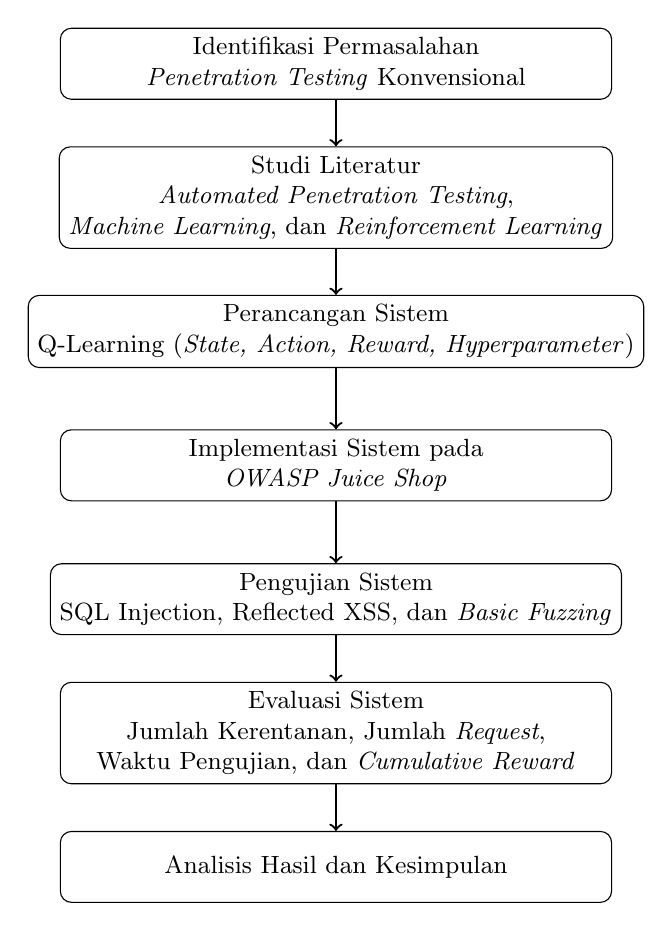
\begin{tikzpicture}[
    node distance=1.7cm,
    every node/.style={font=\small},
    process/.style={
        rectangle,
        draw=black,
        rounded corners,
        align=center,
        minimum width=7cm,
        minimum height=0.9cm
    },
    arrow/.style={
        ->,
        thick
    }
]

\node (start) [process] {Identifikasi Permasalahan \\ \textit{Penetration Testing} Konvensional};

\node (literature) [process, below of=start] {Studi Literatur \\ \textit{Automated Penetration Testing}, \\ \textit{Machine Learning}, dan \textit{Reinforcement Learning}};

\node (design) [process, below of=literature] {Perancangan Sistem \\ Q-Learning (\textit{State, Action, Reward, Hyperparameter})};

\node (implementation) [process, below of=design] {Implementasi Sistem pada \\ \textit{OWASP Juice Shop}};

\node (testing) [process, below of=implementation] {Pengujian Sistem \\ SQL Injection, Reflected XSS, dan \textit{Basic Fuzzing}};

\node (evaluation) [process, below of=testing] {Evaluasi Sistem \\ Jumlah Kerentanan, Jumlah \textit{Request}, \\ Waktu Pengujian, dan \textit{Cumulative Reward}};

\node (analysis) [process, below of=evaluation] {Analisis Hasil dan Kesimpulan};

\draw [arrow] (start) -- (literature);
\draw [arrow] (literature) -- (design);
\draw [arrow] (design) -- (implementation);
\draw [arrow] (implementation) -- (testing);
\draw [arrow] (testing) -- (evaluation);
\draw [arrow] (evaluation) -- (analysis);

\end{tikzpicture}
\caption{Alur Penelitian}
\label{fig:alur_penelitian}
\end{figure}

Alur penelitian ini dimulai dari adanya permasalahan pada proses \textit{penetration testing} konvensional yang masih memiliki beberapa keterbatasan. Pengujian secara manual atau berbasis aturan tetap cenderung membutuhkan waktu yang lebih lama, bergantung pada keahlian penguji, dan kurang mampu menyesuaikan diri terhadap kondisi sistem yang berubah.

Berdasarkan permasalahan tersebut, penelitian ini mengusulkan penggunaan \textit{Reinforcement Learning} sebagai pendekatan untuk membantu proses \textit{automated penetration testing}. Melalui pendekatan ini, sistem dirancang agar dapat belajar dari setiap percobaan pengujian yang dilakukan. Agen akan memilih aksi berupa payload tertentu, mengirimkannya ke aplikasi target, kemudian menerima respons dari sistem sebagai dasar untuk menentukan tindakan berikutnya.

Penelitian ini diterapkan pada aplikasi web \textit{OWASP Juice Shop} sebagai lingkungan pengujian. Sistem akan diuji untuk melihat kemampuannya dalam menemukan kerentanan seperti \textit{SQL Injection}, \textit{Reflected Cross-Site Scripting} (Reflected XSS), dan \textit{basic fuzzing}. Hasil pengujian kemudian dievaluasi berdasarkan beberapa metrik, yaitu jumlah kerentanan yang ditemukan, jumlah \textit{request}, waktu pengujian, dan nilai \textit{cumulative reward}.

Dengan alur tersebut, penelitian ini diharapkan dapat menunjukkan apakah pendekatan \textit{Reinforcement Learning} mampu meningkatkan efektivitas dan efisiensi proses \textit{penetration testing} dibandingkan dengan pendekatan konvensional.
